% LNCS-style report (compile on Overleaf with Springer LNCS template)
\documentclass[runningheads]{llncs}

% Packages
\usepackage[T1]{fontenc}
\usepackage{graphicx}
\usepackage{amsmath}
\usepackage{booktabs}
\usepackage[hidelinks]{hyperref}
\usepackage{float}

\begin{document}

\title{Experimental Linear Regression on California Housing}
\titlerunning{Linear Regression on California Housing}

\author{Umer Farooq}
\authorrunning{U. Farooq}
\institute{Section CS-7B, Roll No: 22I-0891}

\maketitle

\pagestyle{plain}

% Increase spacing in tables for readability
\renewcommand{\arraystretch}{1.3}
\setlength{\tabcolsep}{8pt}

\begin{abstract}
We analyze the California Housing dataset using Linear Regression and SGD-based regression, following a five-phase experimental protocol with NumPy and scikit-learn only (no pandas). We report MSE, RMSE, MAE, and $R^2$ consistently, use pipelines for cross-validation, scale inputs for SGD, and summarize EDA insights, strongest correlations, model comparisons, and CV stability.
\keywords{Linear Regression \and SGD Regressor \and California Housing \and Cross-Validation}
\end{abstract}

\section{Introduction}
This work studies linear models on the California Housing dataset with a focus on reproducible experimentation and fair comparison across metrics. The target variable is \texttt{MedHouseVal} (median house value in \$100k USD). We avoid pandas by design, relying on NumPy and scikit-learn for all data manipulation and modeling tasks. Our experimental protocol spans five phases: initial data exploration, single-feature modeling, multi-feature polynomial regression, train-test validation, and cross-validation assessment.

\section{Dataset and Methodology}

\subsection{Dataset}
We use \texttt{sklearn.datasets.fetch\_california\_housing}, which contains 20,640 samples from the 1990 California census. The dataset includes eight features: \texttt{MedInc} (median income), \texttt{HouseAge} (median house age), \texttt{AveRooms} (average number of rooms), \texttt{AveBedrms} (average number of bedrooms), \texttt{Population} (block population), \texttt{AveOccup} (average occupancy), \texttt{Latitude}, and \texttt{Longitude}. The target variable is \texttt{MedHouseVal} (median house value in \$100k). The data matrix has shape $X \in \mathbb{R}^{20640 \times 8}$ and target vector $y \in \mathbb{R}^{20640}$.

\subsection{Metrics}
We compute four standard regression metrics using NumPy implementations: Mean Squared Error (MSE), Root Mean Squared Error (RMSE), Mean Absolute Error (MAE), and coefficient of determination ($R^2$). For cross-validation (5-fold), we report mean $\pm$ standard deviation across folds to assess model stability.

\subsection{Models and Pipelines}
We compare two linear modeling approaches: Ordinary Least Squares (LR via \texttt{LinearRegression}) and stochastic gradient descent (SGD via \texttt{SGDRegressor}). Input features are standardized for SGD using \texttt{StandardScaler}. We also consider polynomial feature expansions (degrees 2 and 3) in multi-feature settings using \texttt{PolynomialFeatures}. Pipelines encapsulate preprocessing and estimators for proper cross-validation.

\paragraph{Practical considerations and issues.}
Early SGD trials were unstable, exhibiting diverging loss or noisy plateaus when features were unscaled or when using aggressive step sizes. We stabilized training by standardizing inputs, using a conservative constant learning rate ($\eta = 5 \times 10^{-4}$), enabling early stopping with validation monitoring, and employing the robust Huber loss function. These changes improved convergence reliability and brought SGD performance closer to LR on original features.

\section{Exploratory Data Analysis}

\subsection{Descriptive Statistics and Skewness}
We compute per-feature mean, median, minimum, maximum, and standard deviation using NumPy, and report the standardized third moment (skewness) to assess distributional symmetry. Table~\ref{tab:desc-stats} presents the descriptive statistics, while Table~\ref{tab:skew} shows skewness values.

Several features exhibit strong positive skew, particularly \texttt{AveRooms} (skewness = 20.70), \texttt{AveBedrms} (skewness = 31.31), and \texttt{AveOccup} (skewness = 97.63). This heavy right tail indicates the presence of outliers and suggests that means are not fully representative of typical values. In response to this distributional asymmetry, we include MAE alongside MSE in our evaluation metrics and emphasize robust optimization strategies for SGD. Key observations include: (i) heavy right tails for room-related features imply that means substantially exceed medians; (ii) extreme outliers motivate the use of robust loss functions (Huber) and feature scaling; (iii) potential multicollinearity among room-related features cautions against naïve interpretation of individual coefficients.

\begin{table}[H]
  \centering
  \caption{Descriptive statistics per feature (from NumPy).}
  \label{tab:desc-stats}
  \begin{tabular}{lccccc}
    \toprule
    Feature & Mean & Median & Min & Max & Std \\
    \midrule
    MedInc    & 3.8707  & 3.5348  & 0.4999   & 15.0001   & 1.8998 \\
    HouseAge  & 28.6395 & 29.0000 & 1.0000   & 52.0000   & 12.5853 \\
    AveRooms  & 5.4290  & 5.2291  & 0.8462   & 141.9091  & 2.4741 \\
    AveBedrms & 1.0967  & 1.0488  & 0.3333   & 34.0667   & 0.4739 \\
    Population& 1425.4767 & 1166.0000 & 3.0000 & 35682.0000 & 1132.4347 \\
    AveOccup  & 3.0707  & 2.8181  & 0.6923   & 1243.3333 & 10.3858 \\
    Latitude  & 35.6319 & 34.2600 & 32.5400  & 41.9500   & 2.1359 \\
    Longitude & -119.5697 & -118.4900 & -124.3500 & -114.3100 & 2.0035 \\
    \bottomrule
  \end{tabular}
\end{table}

\begin{table}[H]
  \centering
  \caption{Skewness per feature (standardized third moment).}
  \label{tab:skew}
  \begin{tabular}{lc}
    \toprule
    Feature & Skewness \\
    \midrule
    MedInc    & 1.6465 \\
    HouseAge  & 0.0603 \\
    AveRooms  & 20.6964 \\
    AveBedrms & 31.3147 \\
    Population& 4.9355 \\
    AveOccup  & 97.6325 \\
    Latitude  & 0.4659 \\
    Longitude & -0.2978 \\
    \bottomrule
  \end{tabular}
\end{table}

\subsection{Correlations}
We compute Pearson correlation coefficients between each feature and the target variable to identify the most predictive features. Figure~\ref{fig:phase2-eda} provides an overview of feature distributions, while Figure~\ref{fig:phase2-corr} displays the complete correlation matrix as a heatmap.

Table~\ref{tab:corr-target} reveals that \texttt{MedInc} exhibits the strongest linear relationship with \texttt{MedHouseVal} ($r = 0.6881$), suggesting median income is the primary driver of house values in this dataset. Other features show weaker correlations: \texttt{AveRooms} ($r = 0.1519$) and \texttt{HouseAge} ($r = 0.1056$) have modest positive associations, while \texttt{Latitude} ($r = -0.1442$) shows a weak negative correlation, likely reflecting geographic price gradients across California. The remaining features (\texttt{AveBedrms}, \texttt{Longitude}, \texttt{Population}, \texttt{AveOccup}) exhibit very weak correlations with the target, suggesting limited individual predictive power.

\begin{figure}[H]
  \centering
  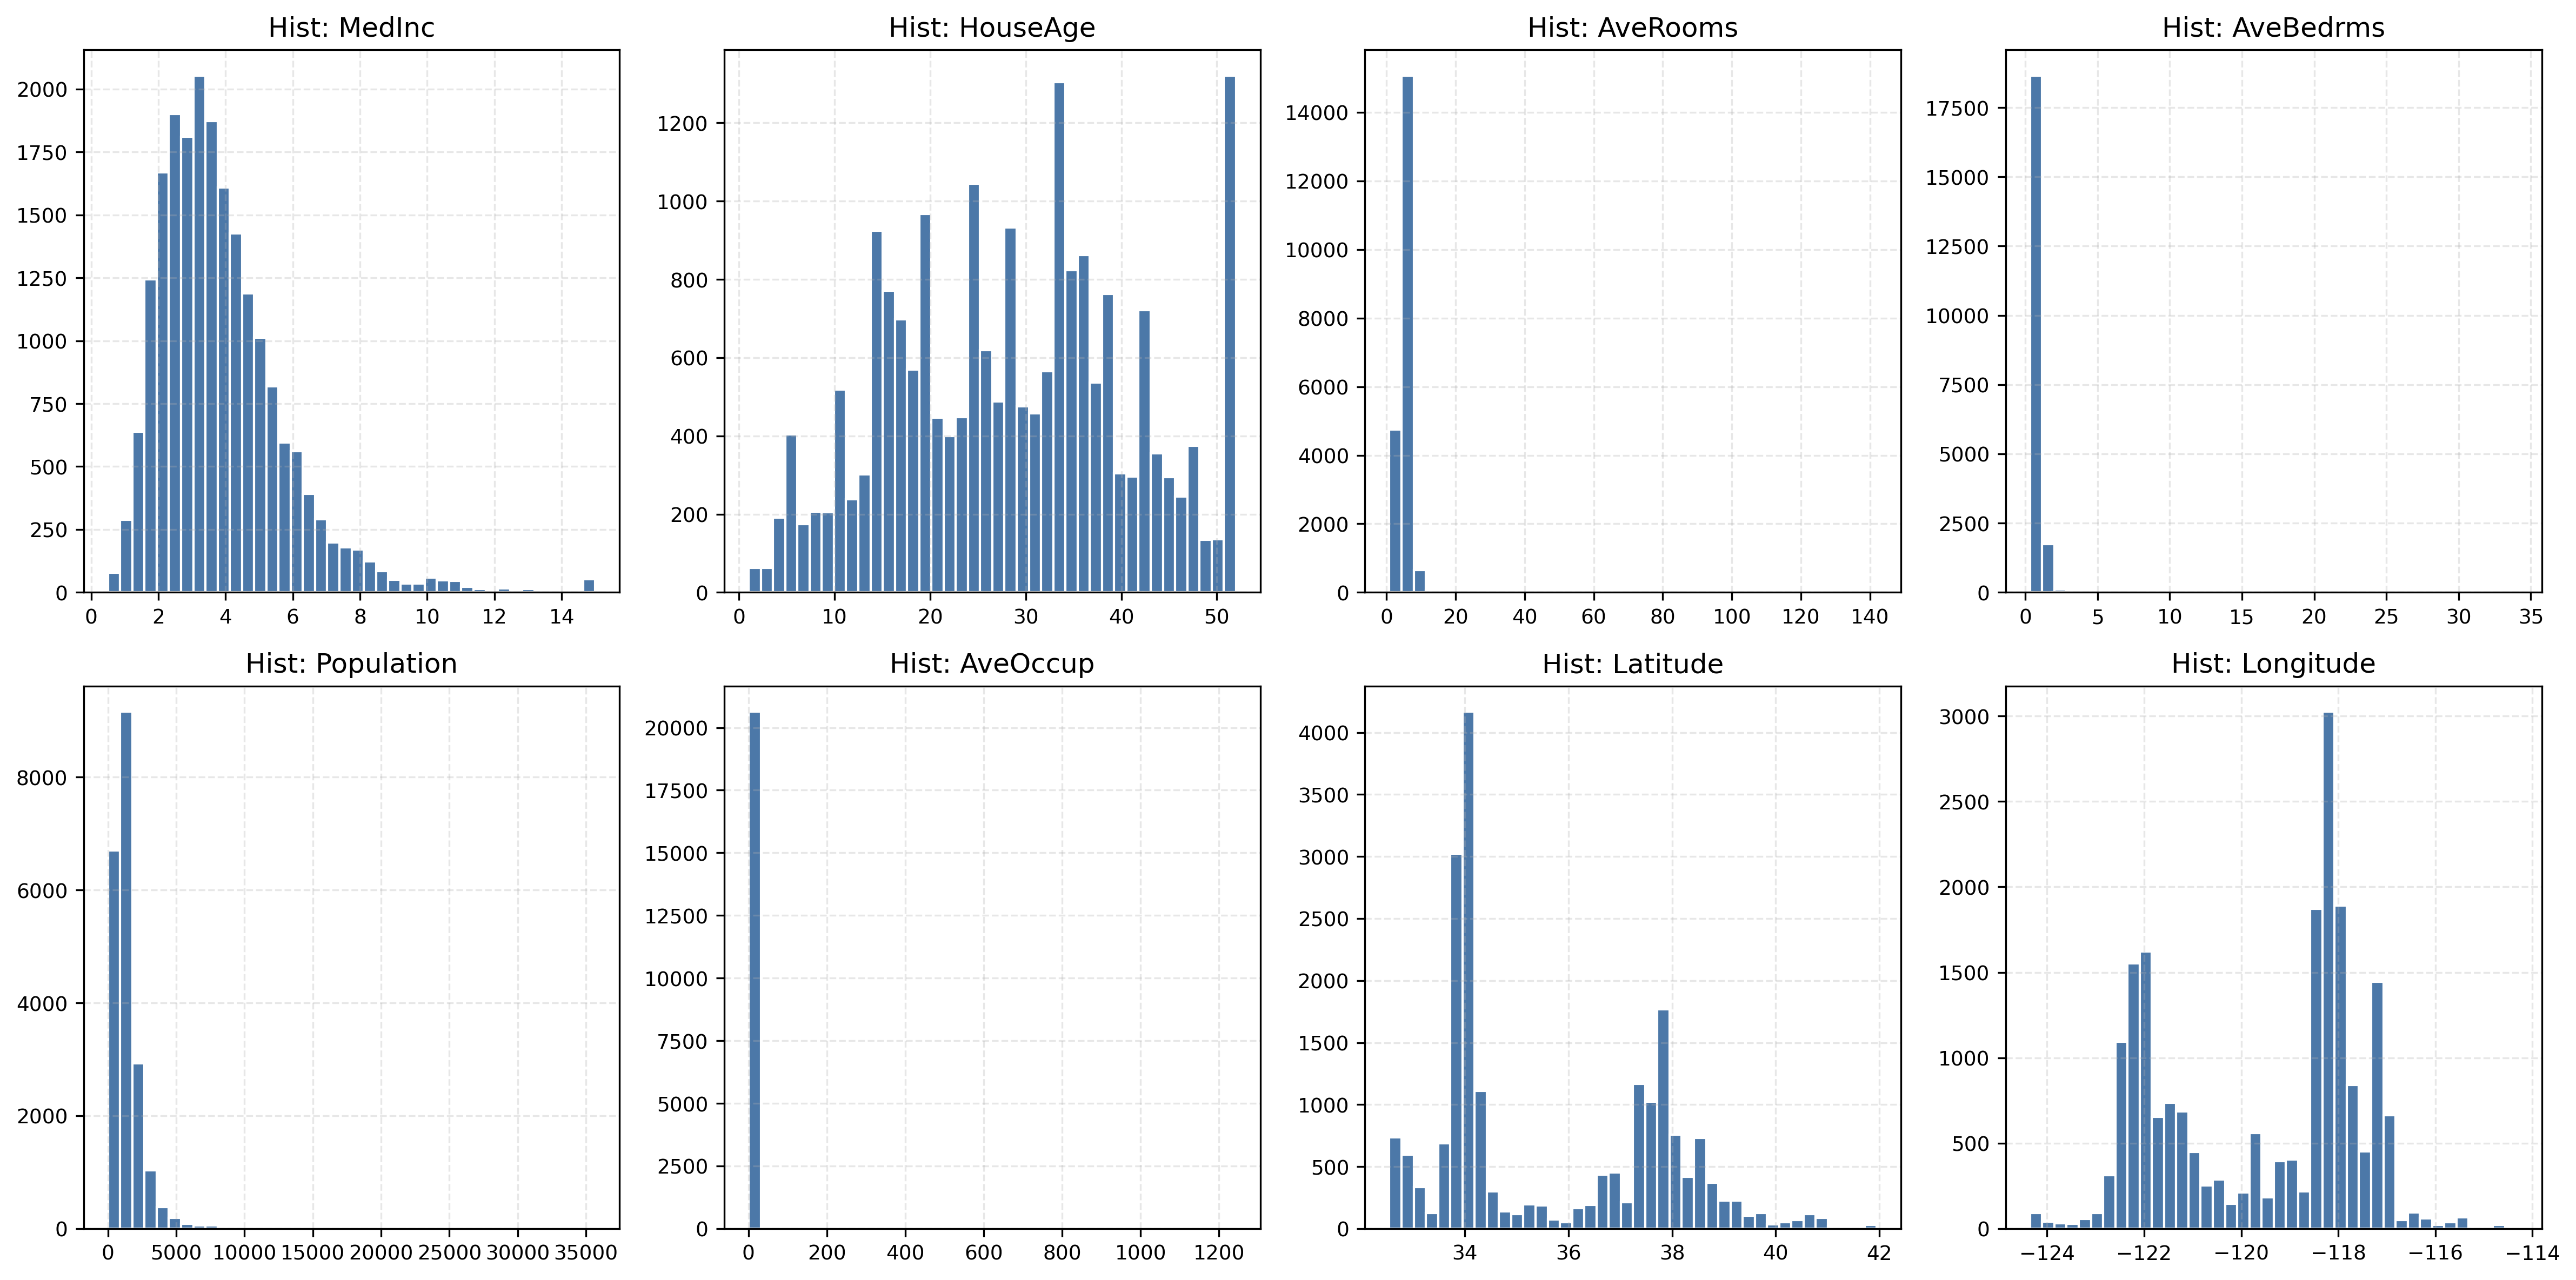
\includegraphics[width=\linewidth]{data/Phase 2 EDA.png}
  \caption{Phase 2 EDA overview (distributions and summaries).}
  \label{fig:phase2-eda}
\end{figure}

\begin{figure}[H]
  \centering
  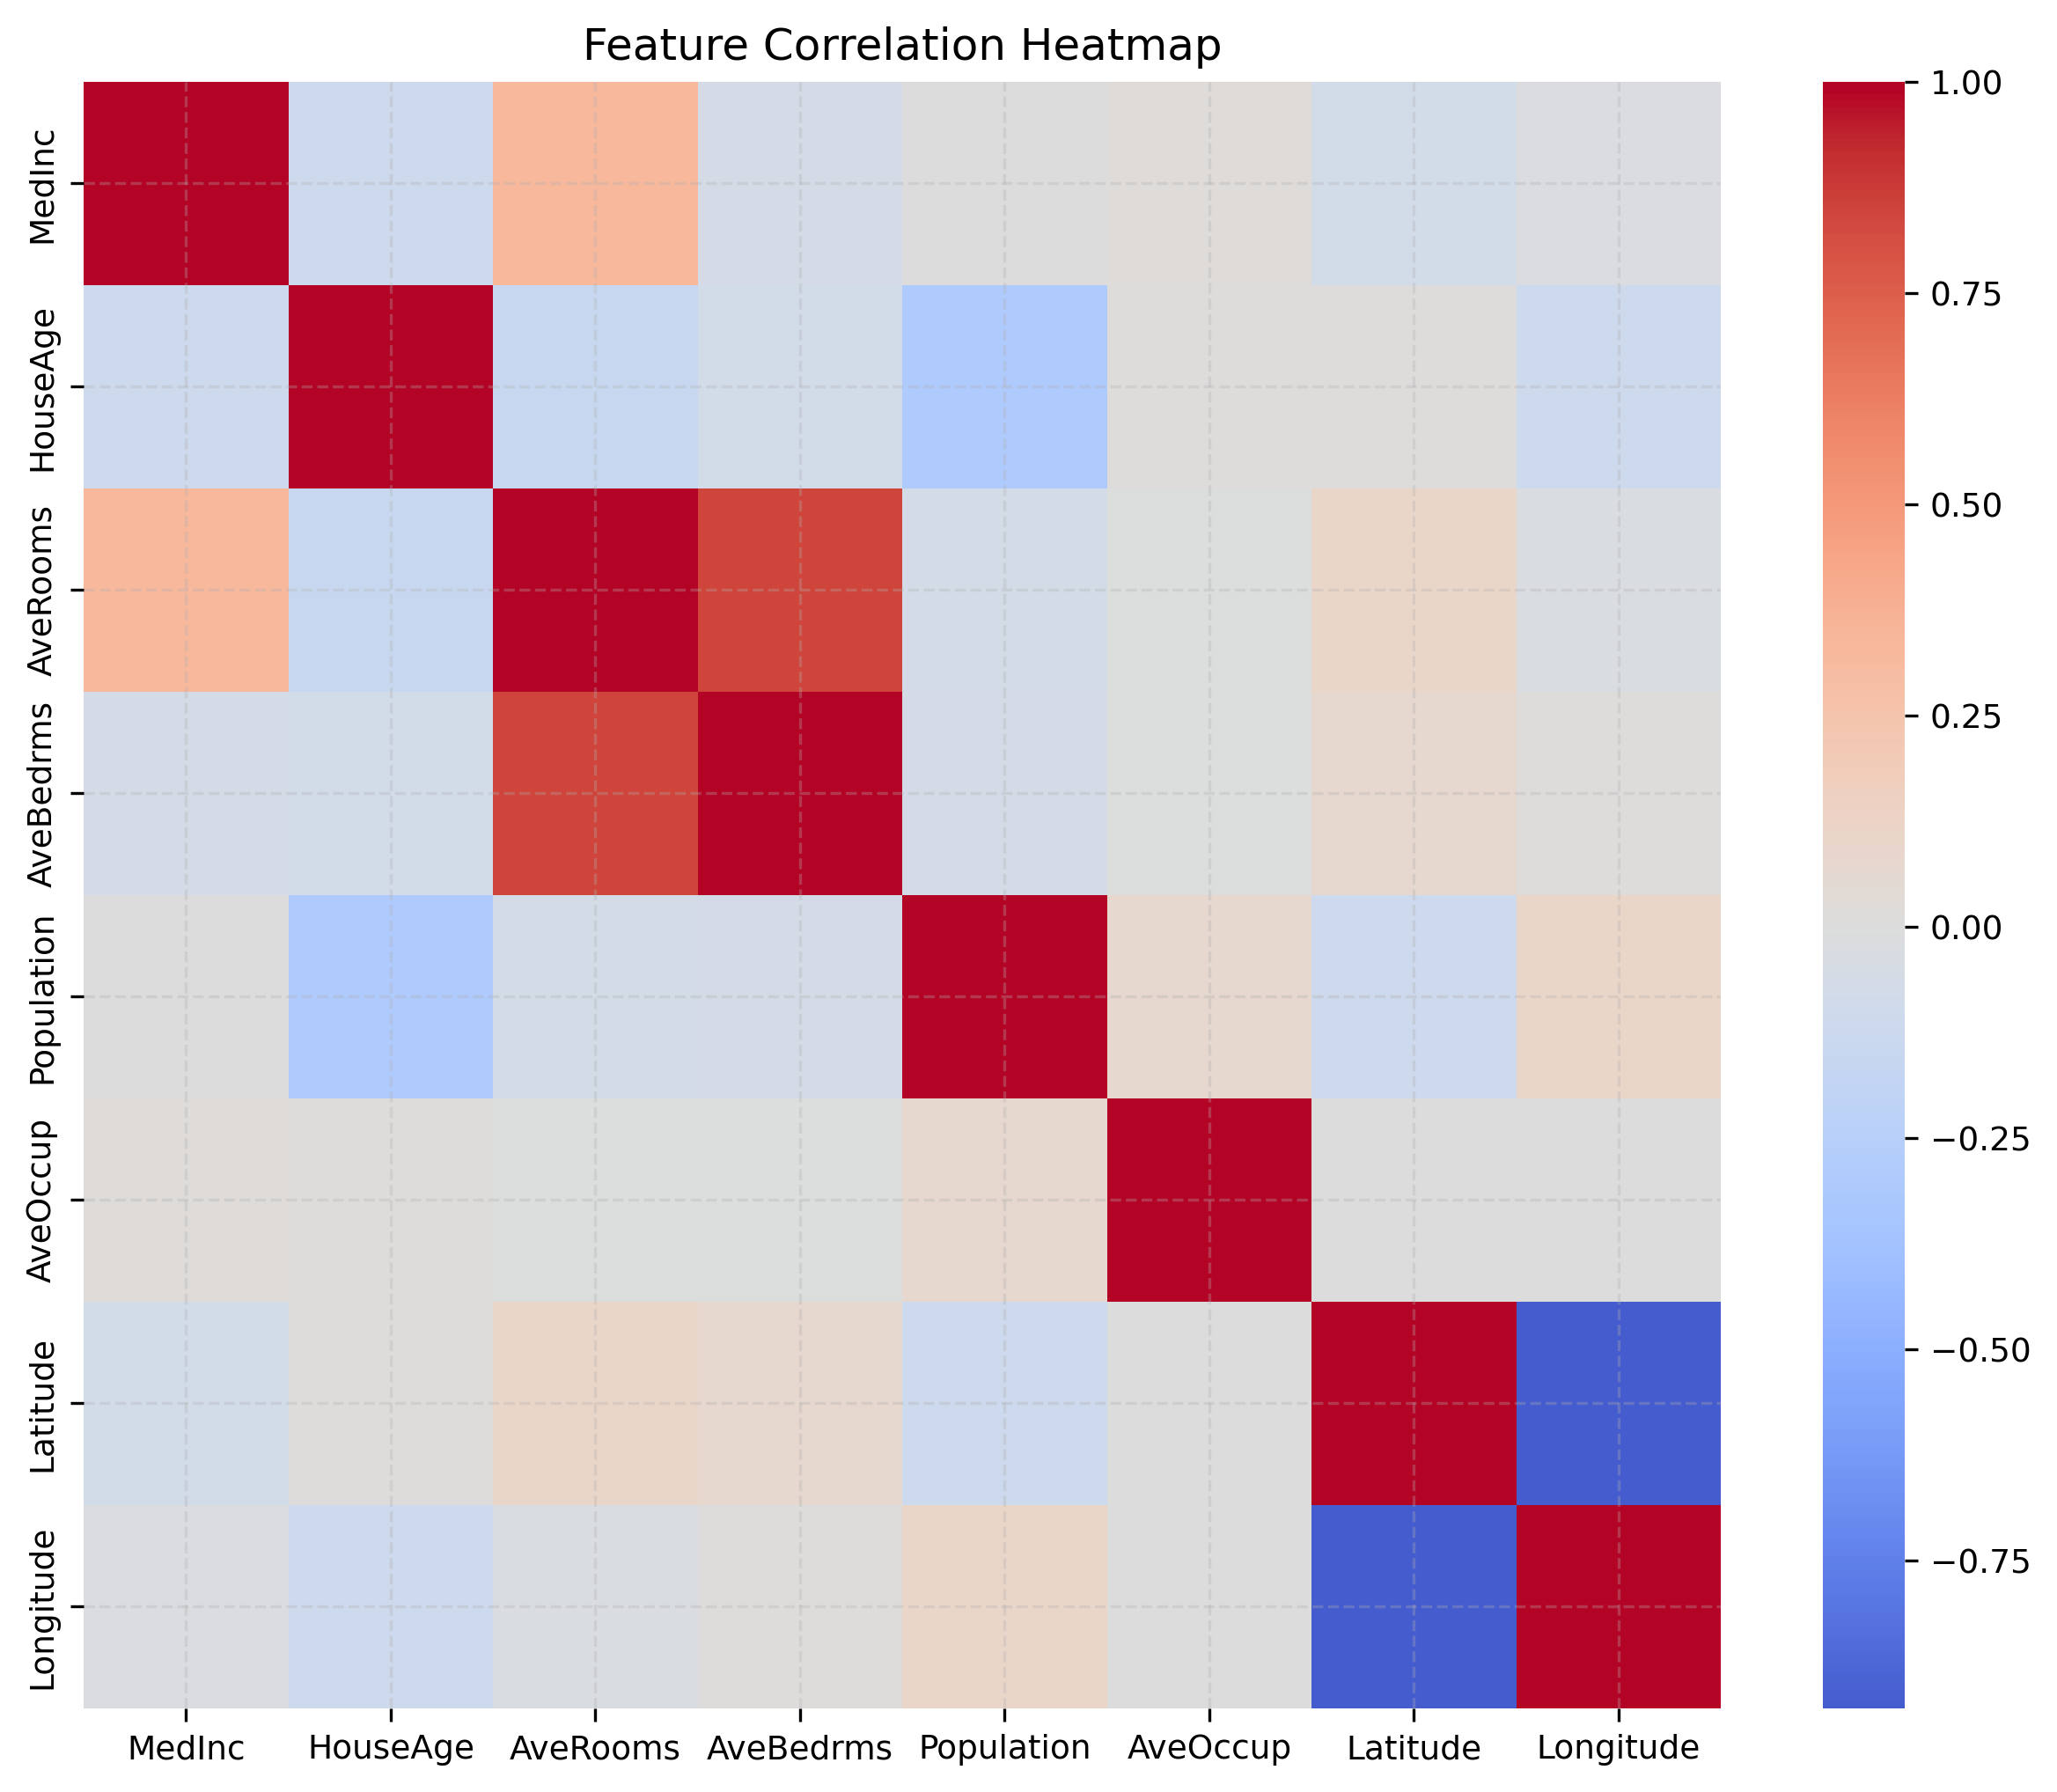
\includegraphics[width=0.95\linewidth]{data/Phase 2 Correlation.png}
  \caption{Feature correlation heatmap. MedInc shows the strongest correlation with MedHouseVal.}
  \label{fig:phase2-corr}
\end{figure}

\begin{table}[H]
  \centering
  \caption{Pearson correlation of each feature with the target (MedHouseVal).}
  \label{tab:corr-target}
  \begin{tabular}{lc}
    \toprule
    Feature & $r$ with target \\
    \midrule
    MedInc    & 0.6881 \\
    AveRooms  & 0.1519 \\
    Latitude  & -0.1442 \\
    HouseAge  & 0.1056 \\
    AveBedrms & -0.0467 \\
    Longitude & -0.0460 \\
    Population& -0.0246 \\
    AveOccup  & -0.0237 \\
    \bottomrule
  \end{tabular}
\end{table}

\section{Experiments}

\subsection{Phase 3A: Single-Feature Regression}
Based on the correlation analysis, we select the strongest predictor (\texttt{MedInc}) for univariate regression. Figure~\ref{fig:3a-scatter} shows the scatter plot with the fitted regression line, demonstrating a clear positive linear trend. Figure~\ref{fig:3a-metrics} compares the performance metrics between LR and SGD.

Table~\ref{tab:3a} presents the in-sample metrics. Linear regression achieves MSE = 0.7011 and $R^2 = 0.4734$, explaining approximately 47\% of variance in house values using median income alone. SGD performs slightly worse (MSE = 0.8234, $R^2 = 0.3816$) due to its approximate optimization nature. The 10 percentage point difference in $R^2$ reflects the gap between exact least-squares solution and iterative gradient-based approximation. Both models achieve similar MAE values (0.6263 vs 0.6327), suggesting comparable typical prediction errors.

\begin{figure}[H]
  \centering
  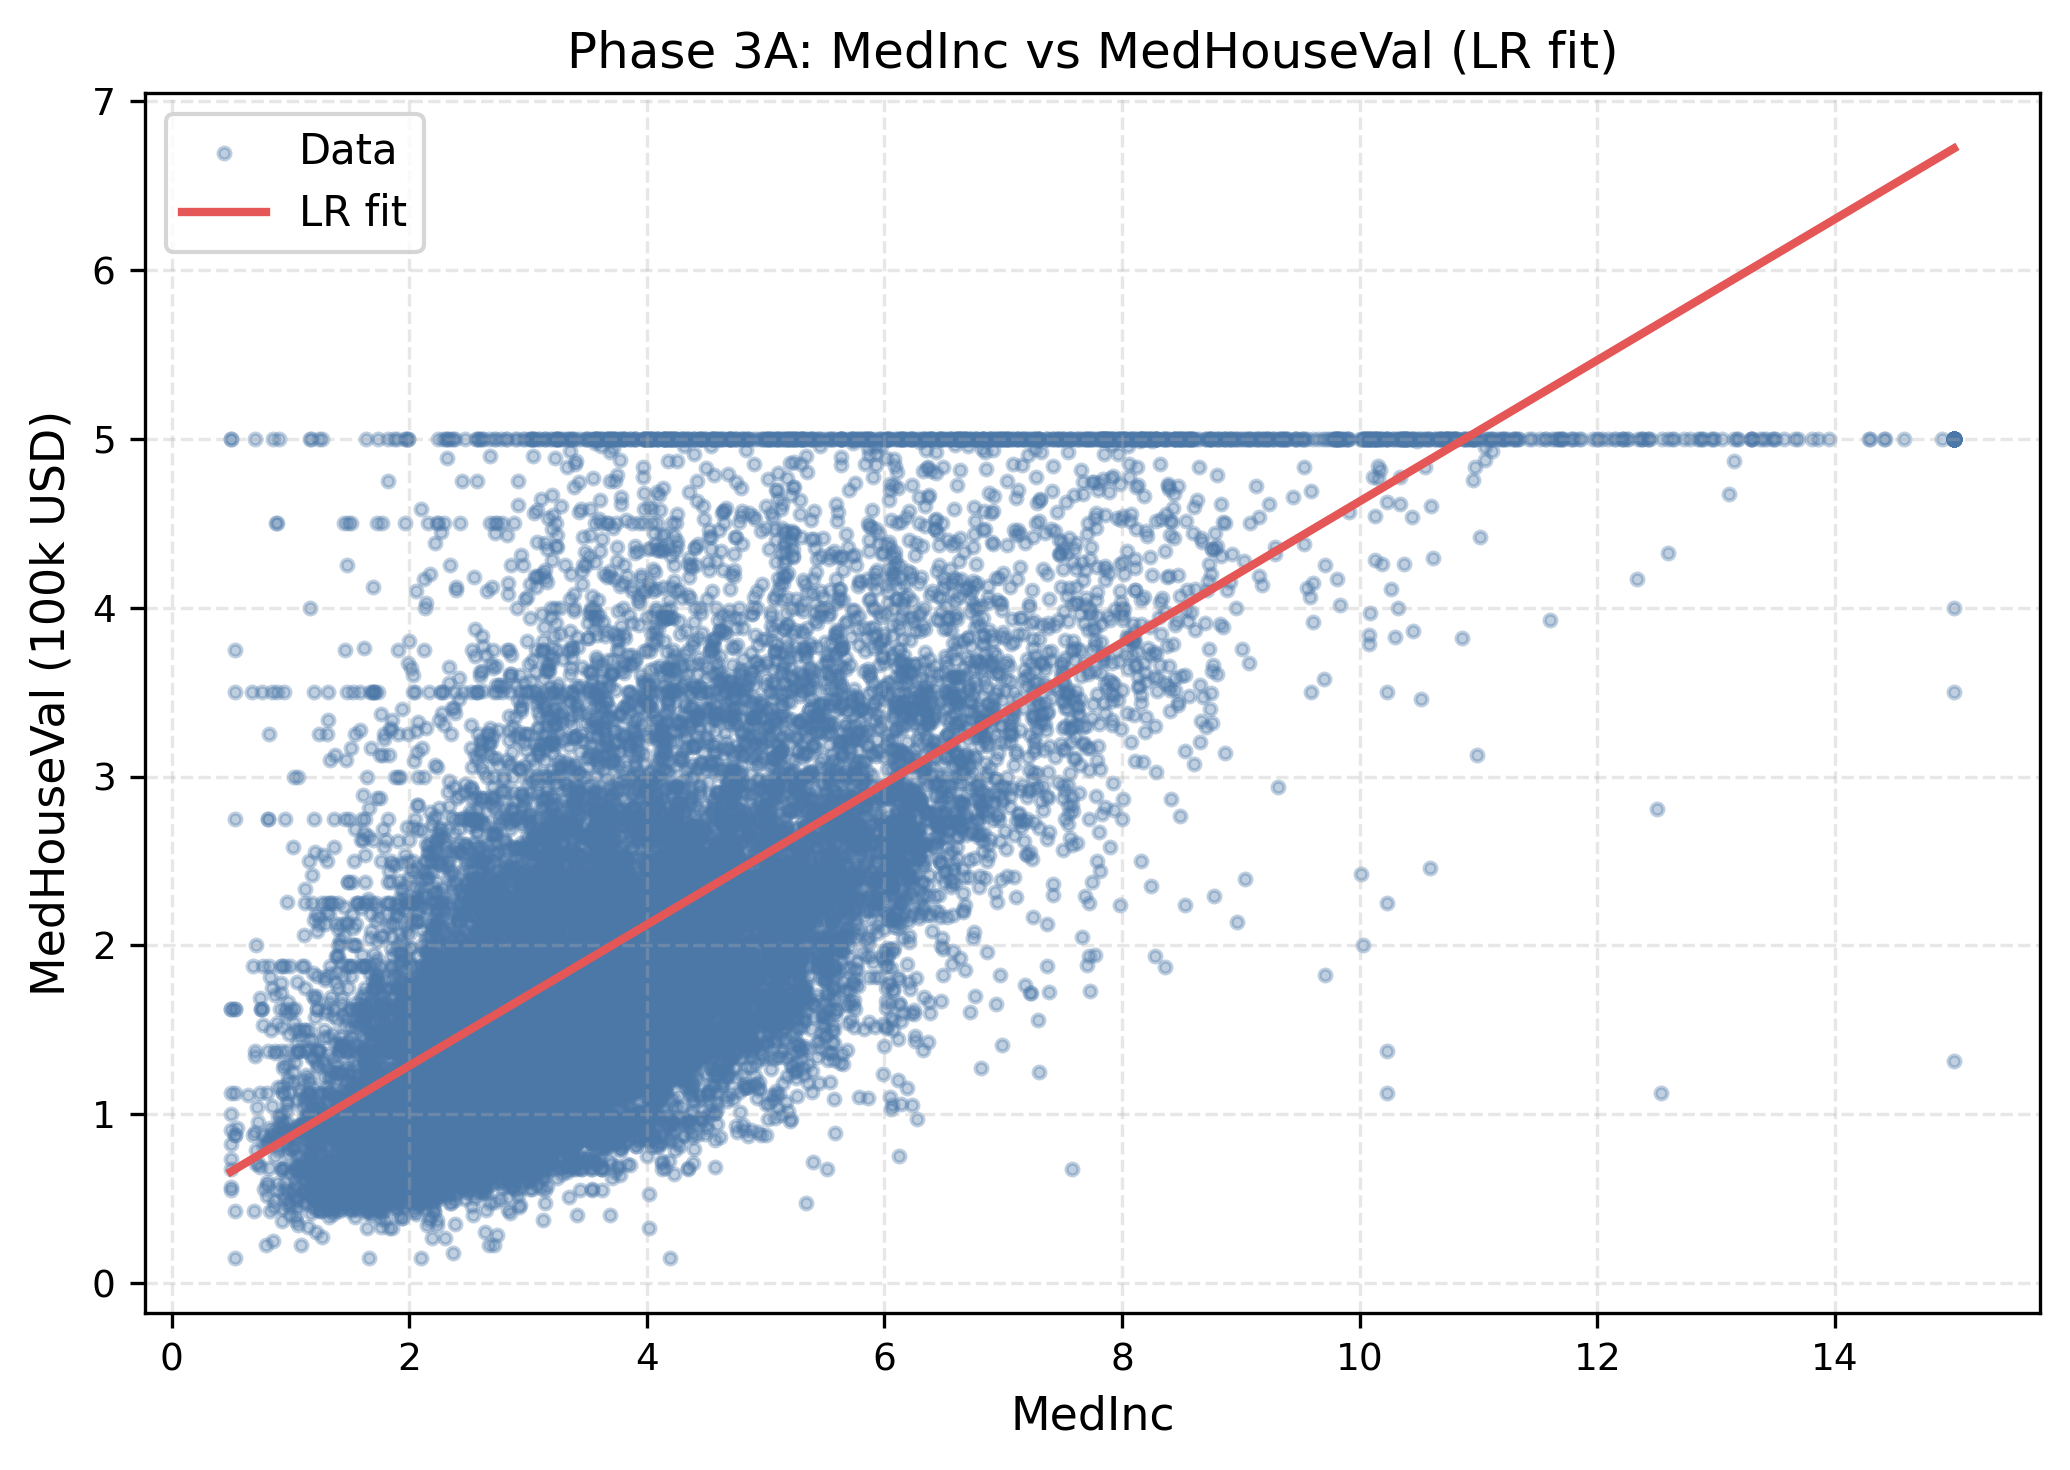
\includegraphics[width=0.9\linewidth]{data/Phase 3A MedInc vs MidHouseVal.png}
  \caption{Single-feature LR: MedInc vs MedHouseVal with fitted line.}
  \label{fig:3a-scatter}
\end{figure}

\begin{figure}[H]
  \centering
  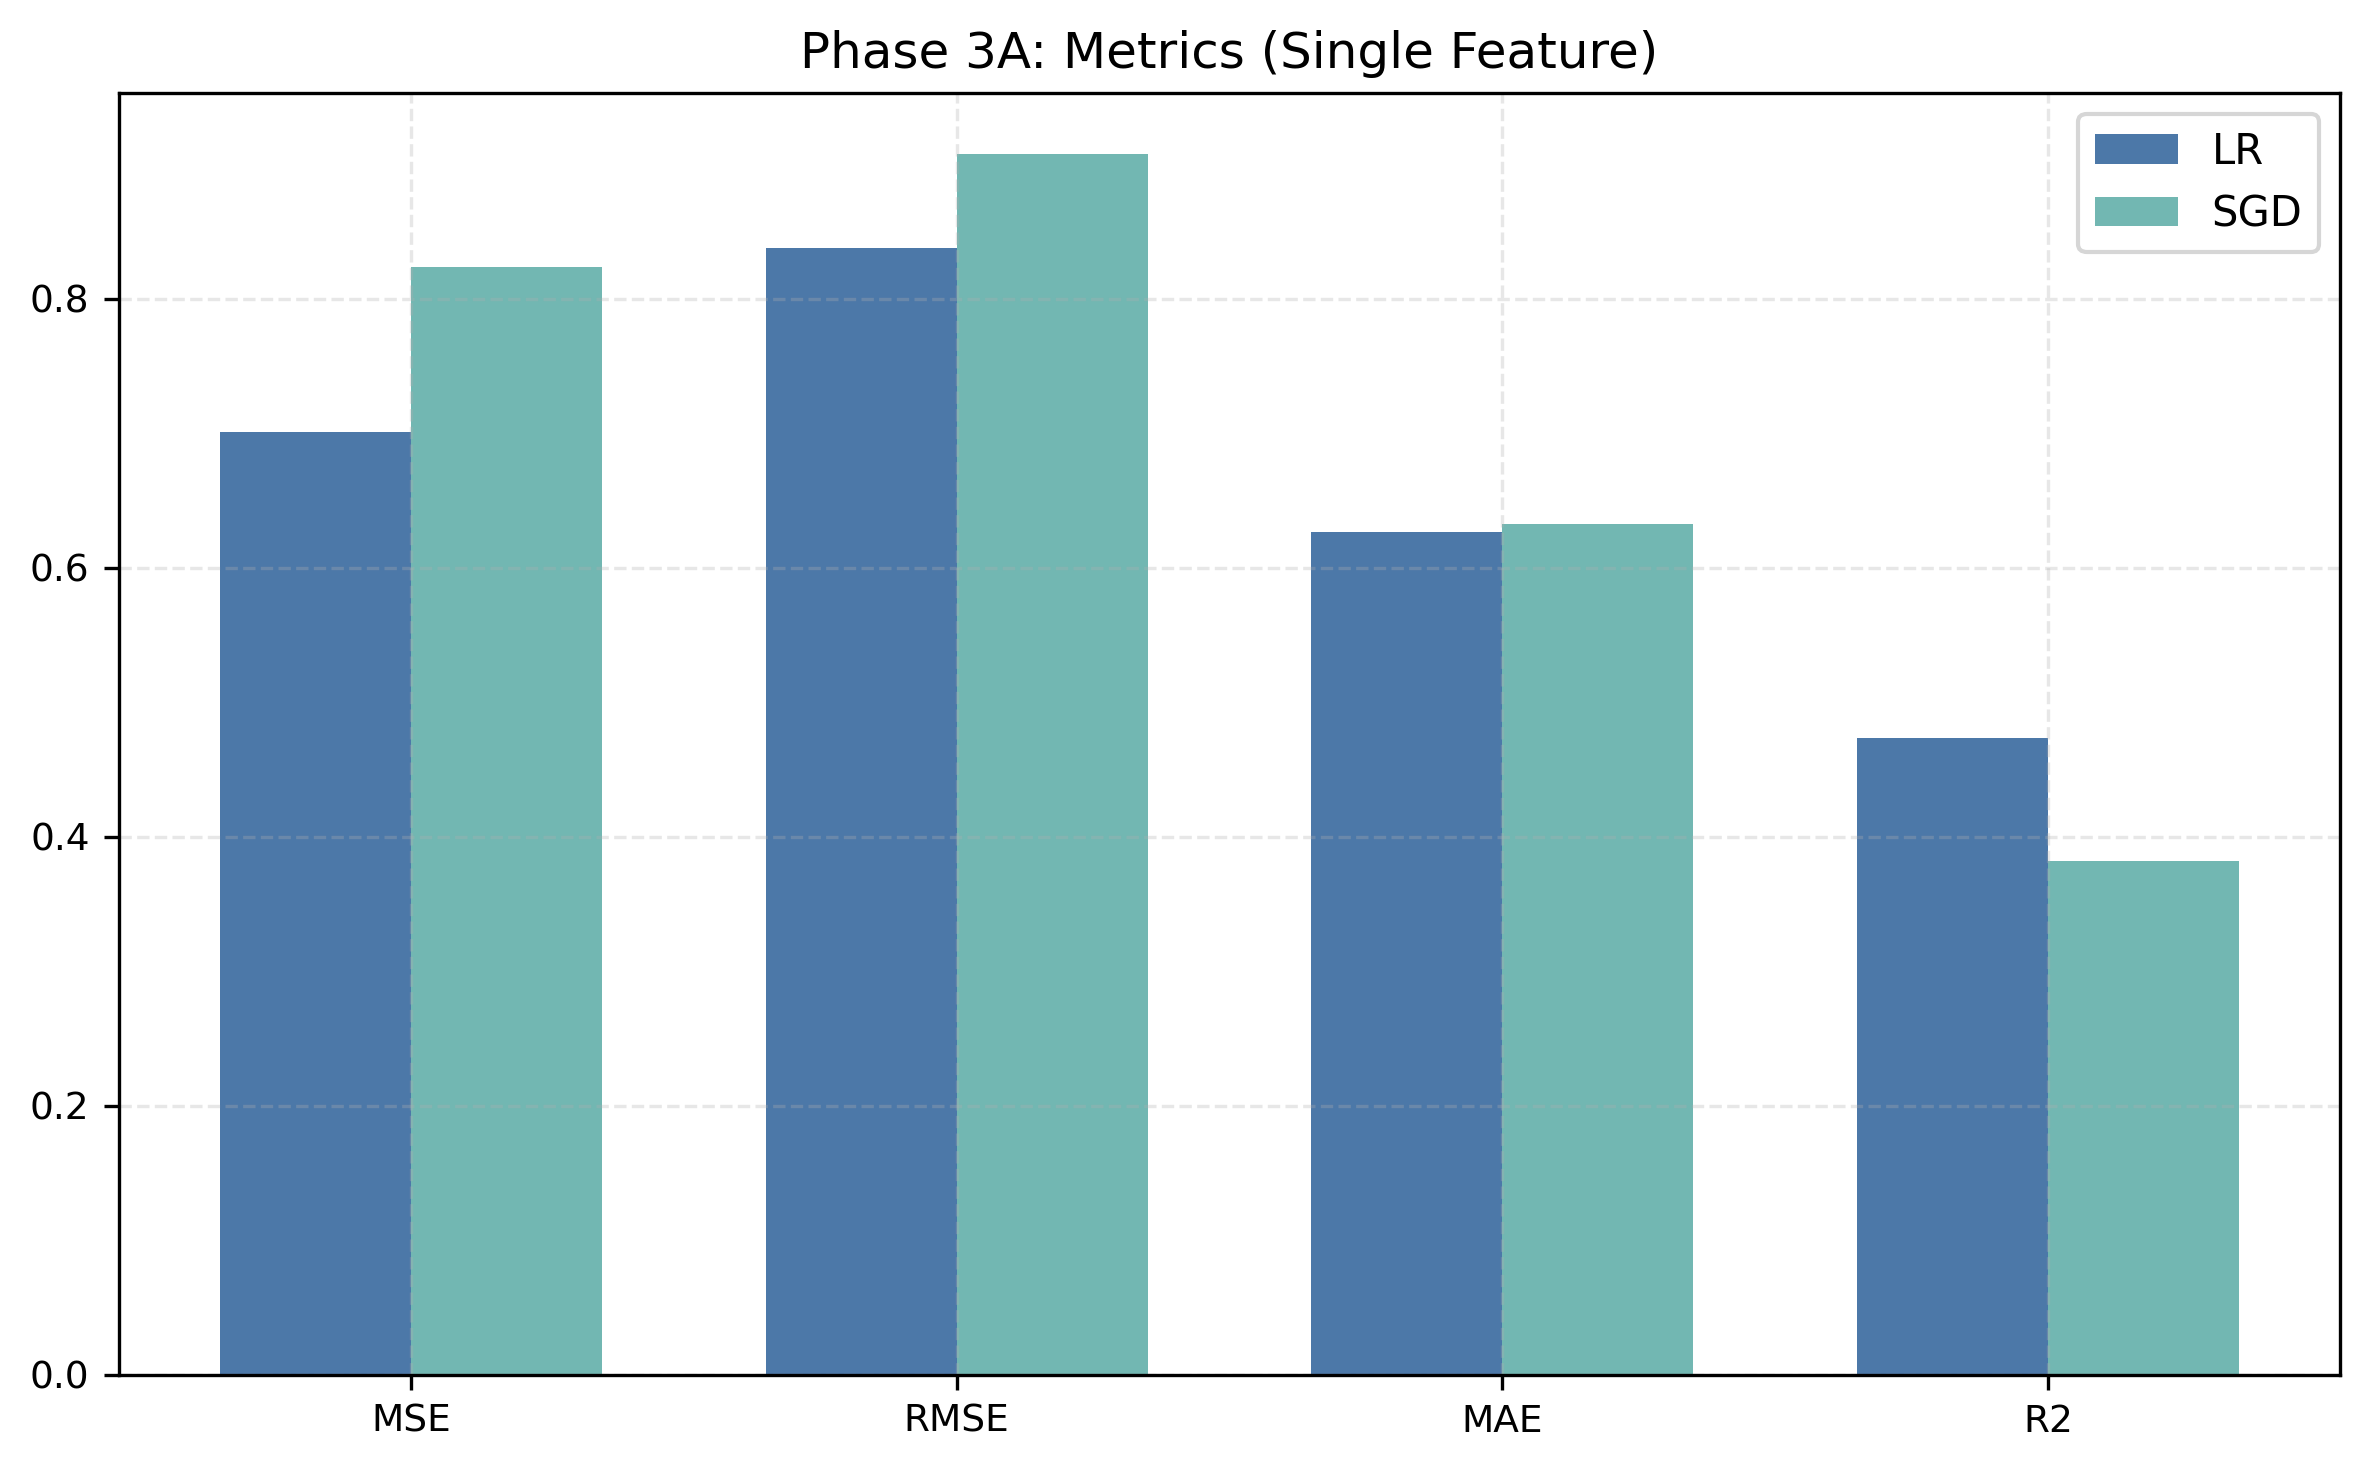
\includegraphics[width=0.9\linewidth]{data/Phase 3A Metrics.png}
  \caption{Phase 3A metrics comparison: LR vs scaled SGD.}
  \label{fig:3a-metrics}
\end{figure}

\begin{table}[H]
  \centering
  \caption{Phase 3A in-sample metrics (single feature: MedInc).}
  \label{tab:3a}
  \begin{tabular}{lcccc}
    \toprule
    Model & MSE & RMSE & MAE & $R^2$ \\
    \midrule
    Single (MedInc) -- LR  & 0.7011 & 0.8373 & 0.6263 & 0.4734 \\
    Single (MedInc) -- SGD & 0.8234 & 0.9074 & 0.6327 & 0.3816 \\
    \bottomrule
  \end{tabular}
\end{table}

\subsection{Phase 3B: Multi-Feature with Polynomial Features}
We evaluate polynomial feature expansions of degrees 1--3 using all eight features. Figures~\ref{fig:3b-r2} and~\ref{fig:3b-mse} illustrate how $R^2$ and MSE evolve with polynomial degree for both models.

Table~\ref{tab:3b} shows that incorporating all features (degree 1) substantially improves performance over the single-feature model: LR achieves MSE = 0.5243 and $R^2 = 0.6062$, a 28\% reduction in MSE. Polynomial expansions further enhance in-sample fit for LR, with degree 3 reaching MSE = 0.3613 and $R^2 = 0.7287$. However, these gains come with increased model complexity (from 8 to 165 features) and potential overfitting risk.

SGD shows more modest improvements from polynomial features, achieving MSE = 0.5895 and $R^2 = 0.5573$ at degree 3. The smaller gains suggest SGD may underfit the polynomial feature space or require additional hyperparameter tuning. The performance gap between LR and SGD widens with higher polynomial degrees, indicating that exact optimization becomes increasingly advantageous as feature dimensionality grows.

\begin{figure}[H]
  \centering
  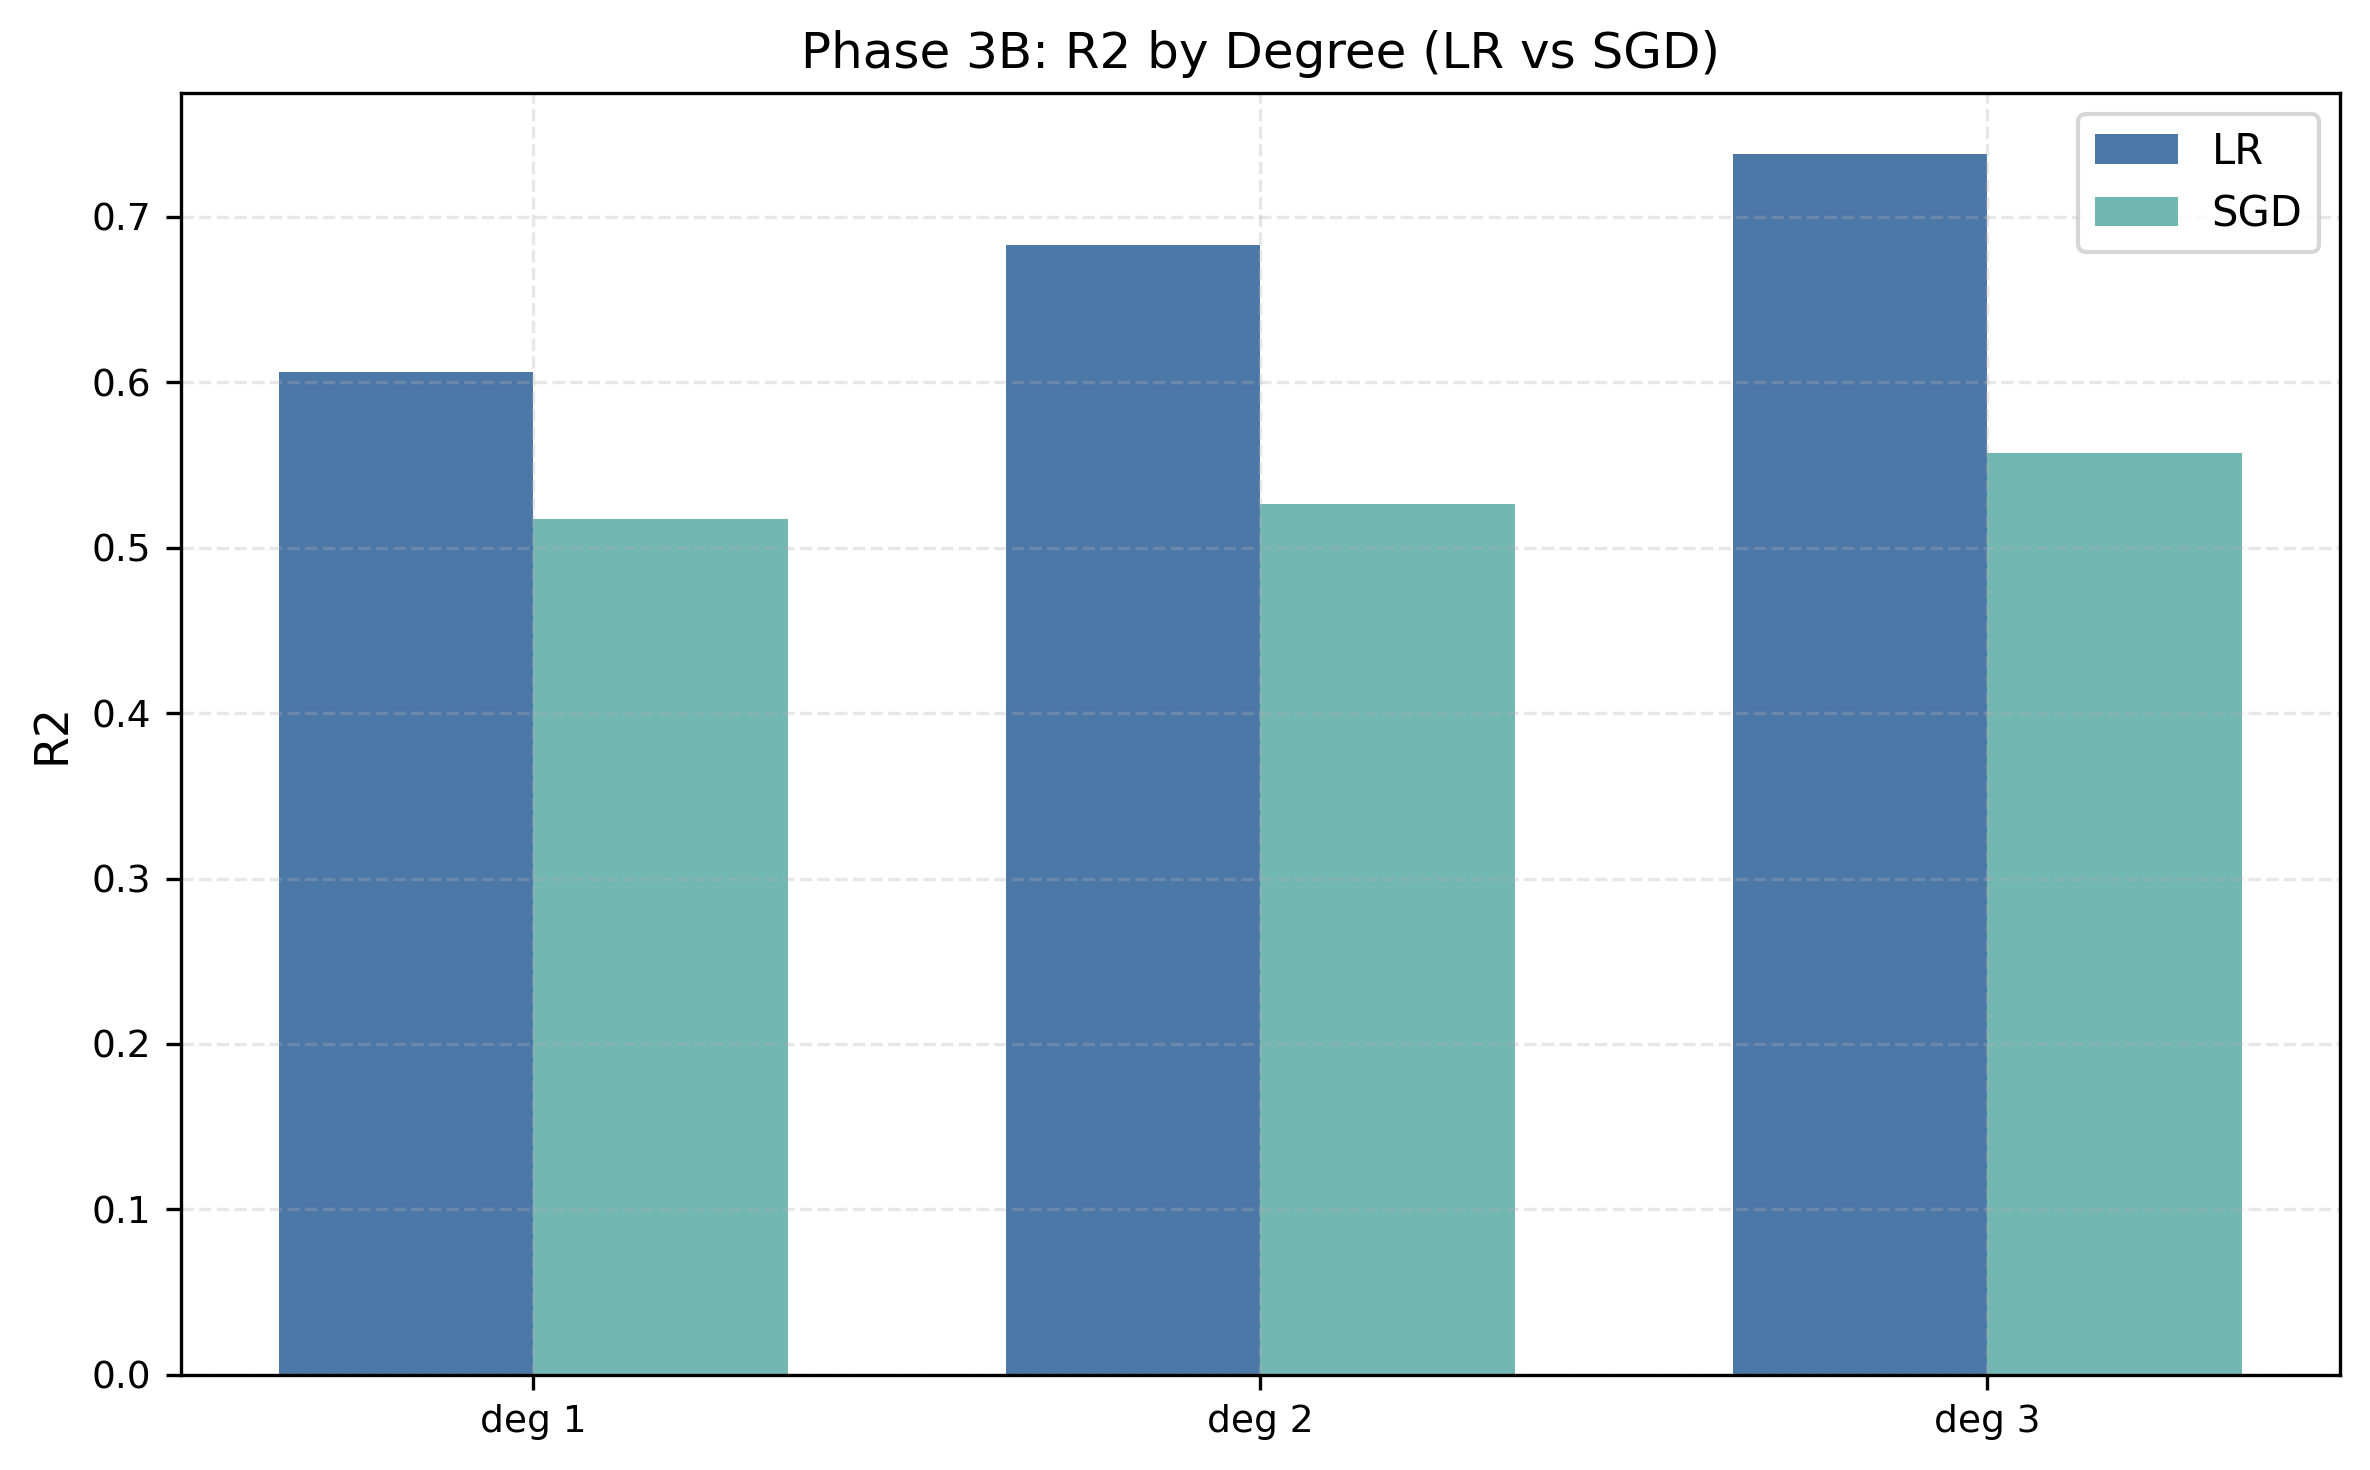
\includegraphics[width=0.9\linewidth]{data/Phase 3B R2.png}
  \caption{Phase 3B: $R^2$ across polynomial degrees for LR and SGD.}
  \label{fig:3b-r2}
\end{figure}

\begin{figure}[H]
  \centering
  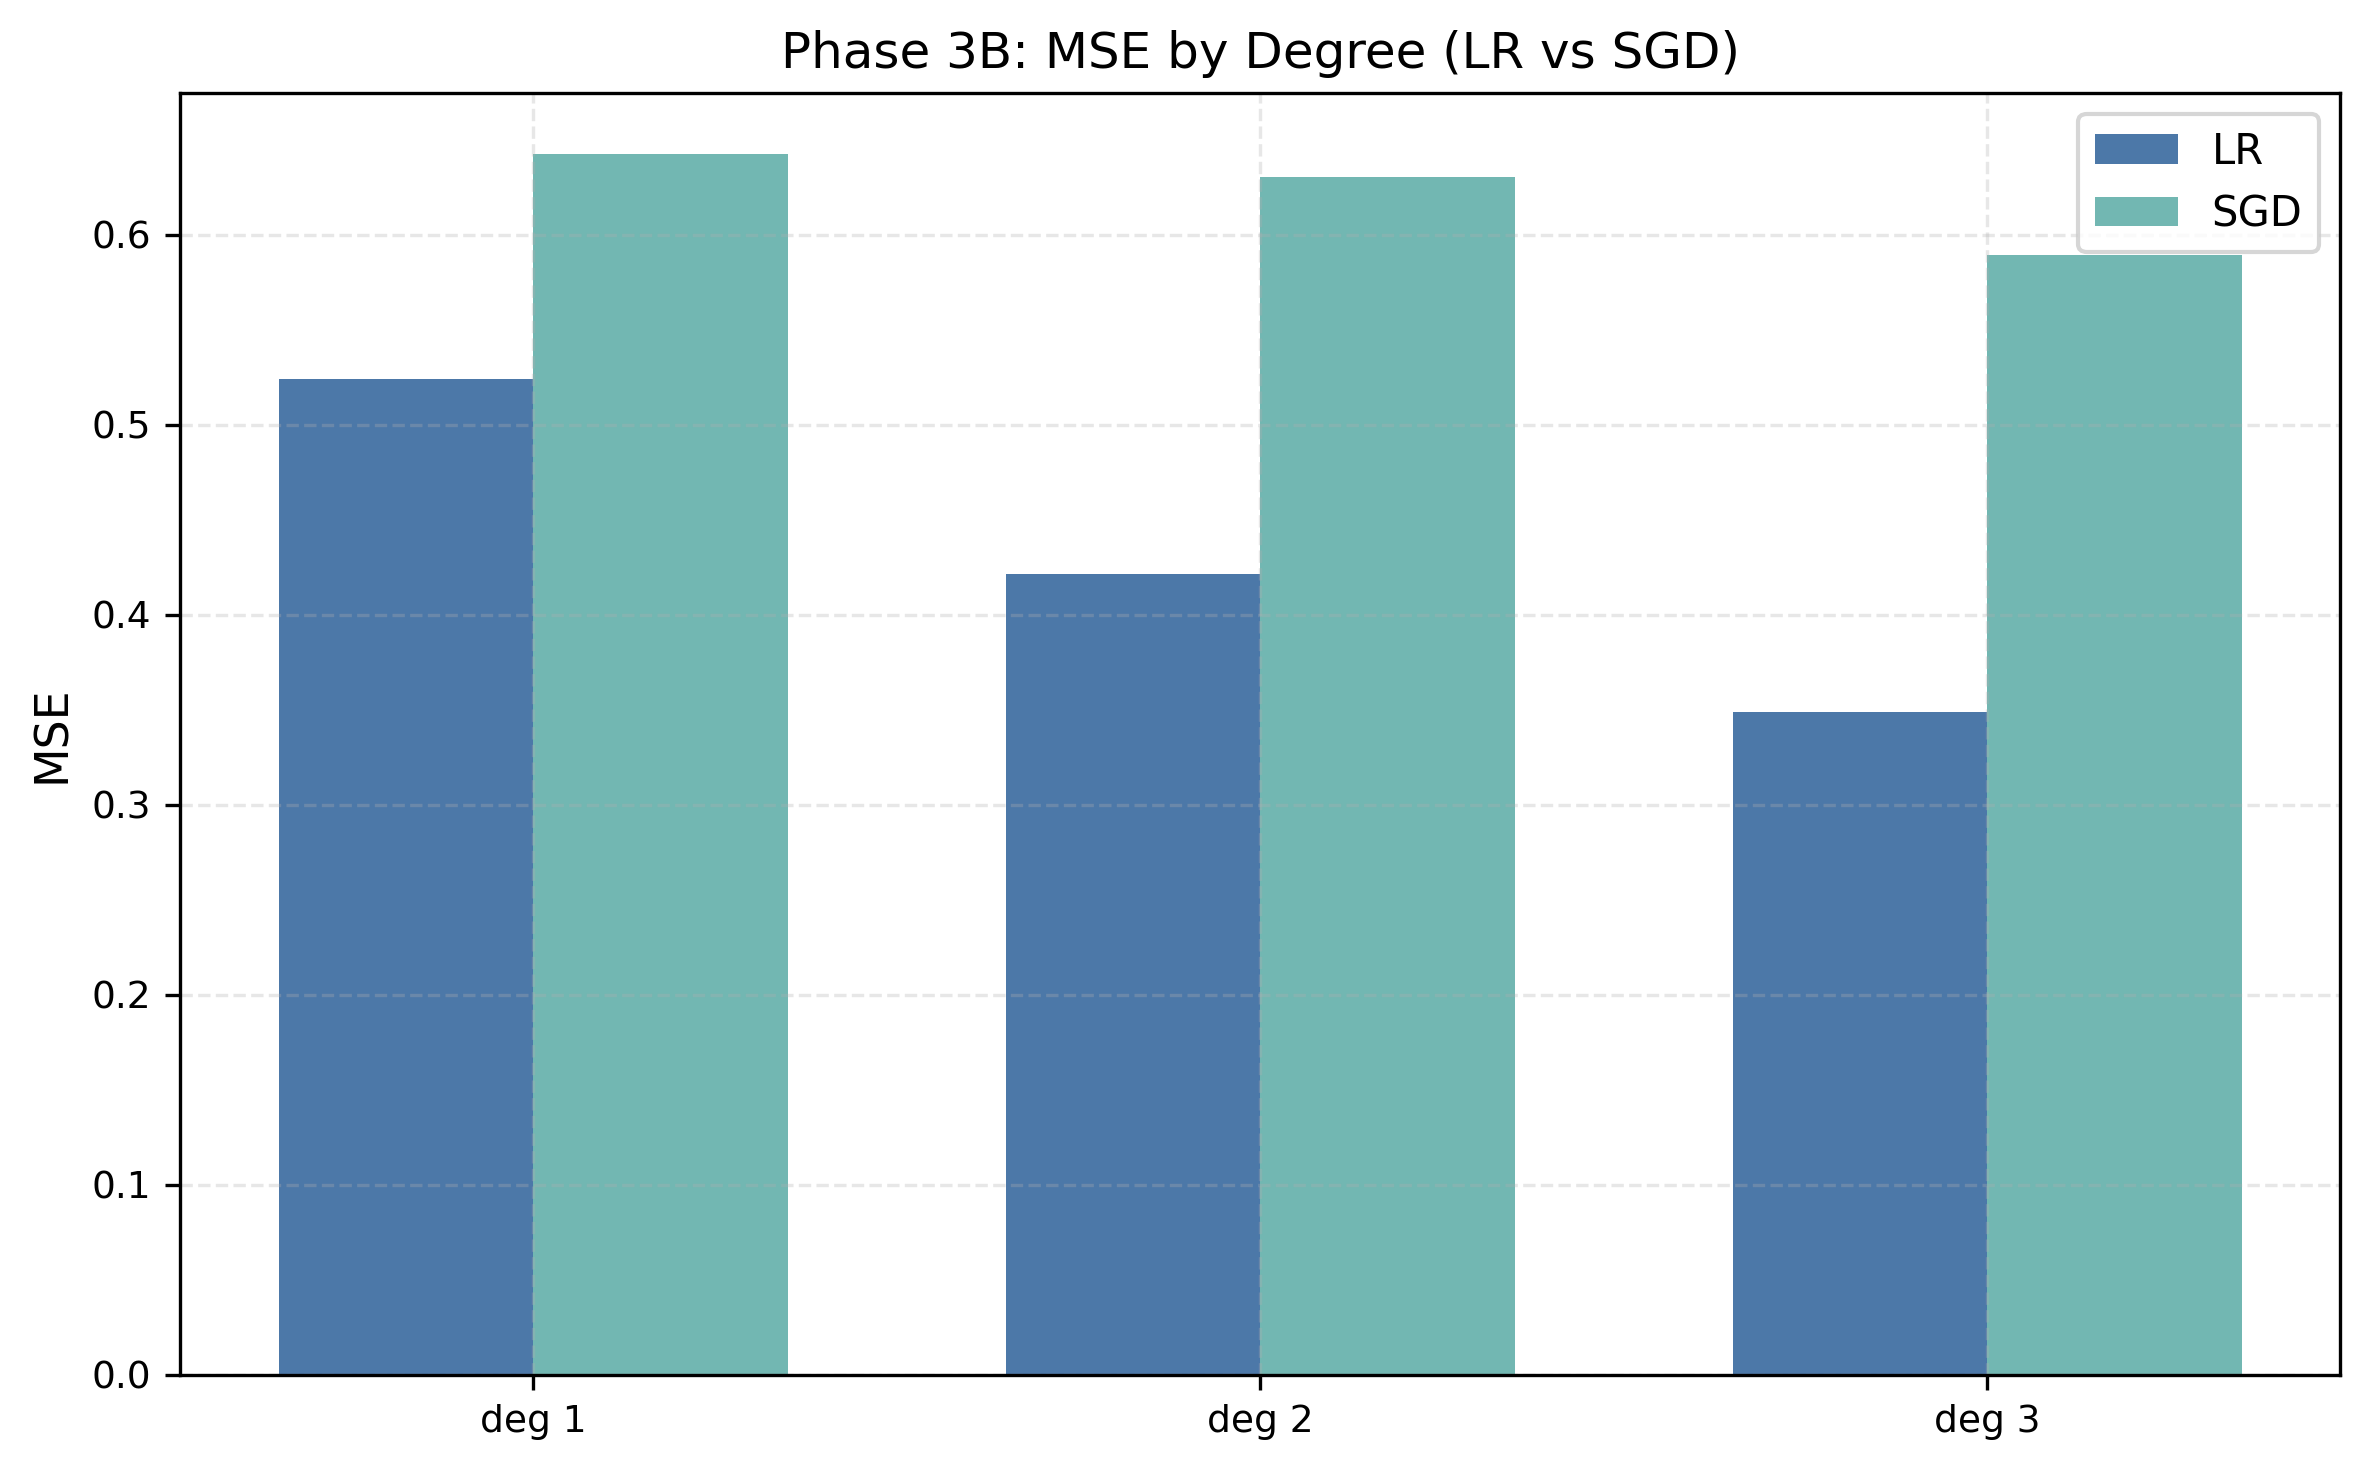
\includegraphics[width=0.9\linewidth]{data/Phase 3B MSE.png}
  \caption{Phase 3B: MSE across polynomial degrees for LR and SGD.}
  \label{fig:3b-mse}
\end{figure}

\begin{table}[H]
  \centering
  \caption{Phase 3B in-sample metrics (all features, polynomial degrees).}
  \label{tab:3b}
  \begin{tabular}{lcccc}
    \toprule
    Model & MSE & RMSE & MAE & $R^2$ \\
    \midrule
    deg 1 -- LR  & 0.5243 & 0.7241 & 0.5312 & 0.6062 \\
    deg 1 -- SGD & 0.6425 & 0.8016 & 0.5459 & 0.5175 \\
    deg 2 -- LR  & 0.4217 & 0.6494 & 0.4614 & 0.6833 \\
    deg 2 -- SGD & 0.6304 & 0.7940 & 0.5299 & 0.5266 \\
    deg 3 -- LR  & 0.3613 & 0.6011 & 0.4284 & 0.7287 \\
    deg 3 -- SGD & 0.5895 & 0.7678 & 0.4989 & 0.5573 \\
    \bottomrule
  \end{tabular}
\end{table}

\subsection{Phase 4: Train/Test Generalization}
We split the data into 80\% training and 20\% testing subsets to assess generalization performance. Both models use only the original eight features (degree 1). Figure~\ref{fig:phase4-residuals} displays residual plots for visual assessment of model fit and heteroscedasticity.

Table~\ref{tab:phase4} reveals small train-test gaps for both models. LR shows test MSE = 0.5559 versus train MSE = 0.5179 (7.3\% increase), while SGD achieves test MSE = 0.5506 versus train MSE = 0.5284 (4.2\% increase). These modest gaps indicate reasonable generalization with minimal overfitting on the original feature set. Notably, SGD slightly outperforms LR on the test set ($R^2 = 0.5798$ vs $0.5758$), suggesting the stochastic optimization may provide implicit regularization benefits. Standardization successfully narrows the performance gap between SGD and LR on held-out data.

\begin{figure}[H]
  \centering
  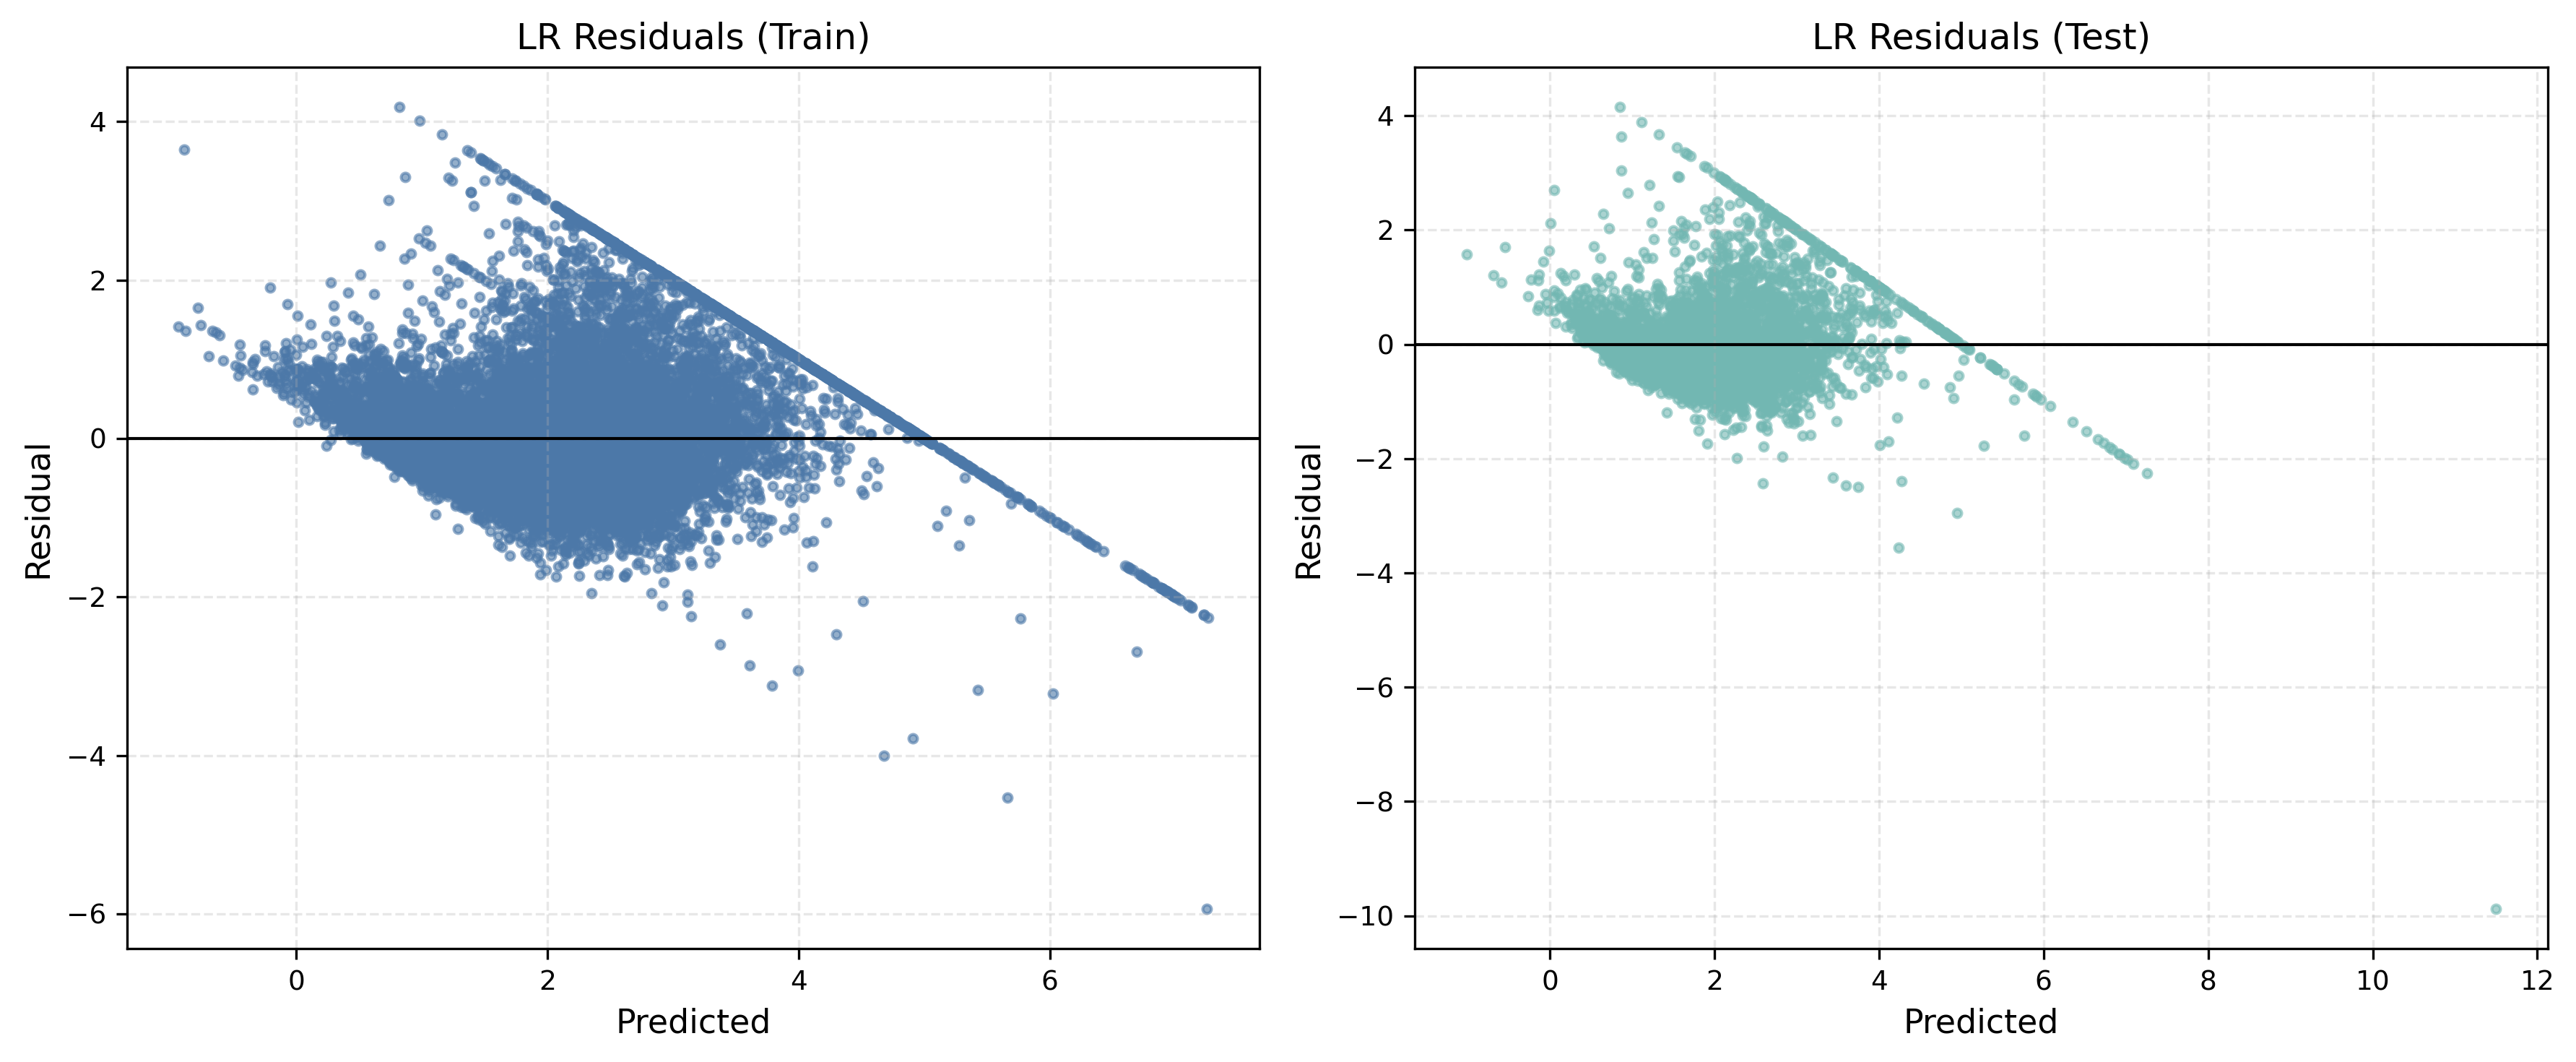
\includegraphics[width=0.49\linewidth]{data/LR Residulas Phase 4.png}\hfill
  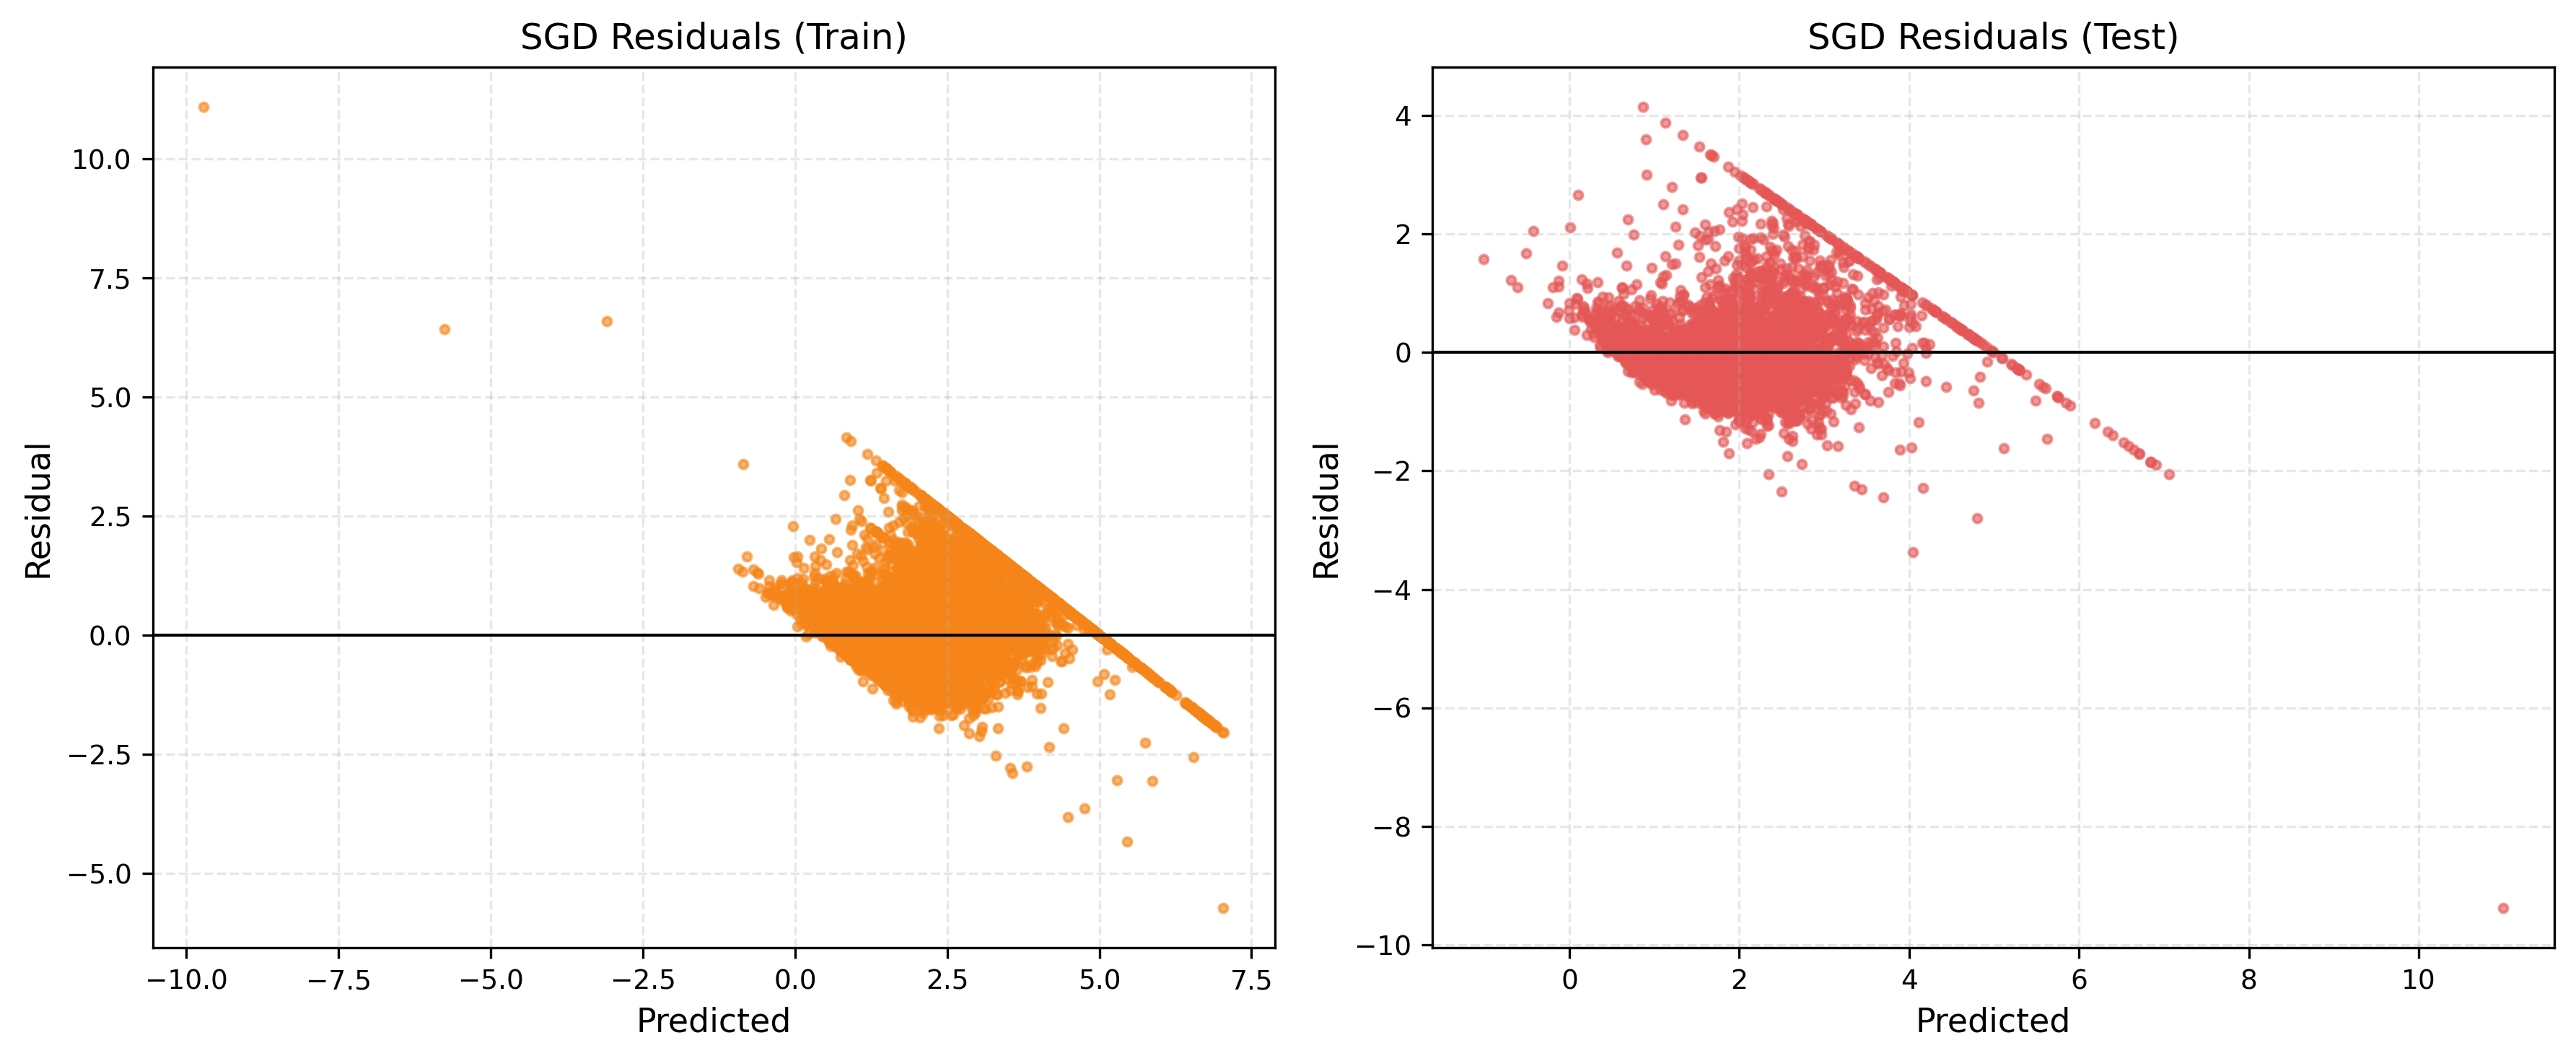
\includegraphics[width=0.49\linewidth]{data/SGD Residulas Phase 4.png}
  \caption{Residual plots for LR (left) and SGD (right) in Phase 4.}
  \label{fig:phase4-residuals}
\end{figure}

\begin{table}[H]
  \centering
  \caption{Phase 4 train/test metrics (80/20 split).}
  \label{tab:phase4}
  \begin{tabular}{lccccc}
    \toprule
    Model & Split & MSE & RMSE & MAE & $R^2$ \\
    \midrule
    LR  & train & 0.5179 & 0.7197 & 0.5286 & 0.6126 \\
    LR  & test  & 0.5559 & 0.7456 & 0.5332 & 0.5758 \\
    SGD & train & 0.5284 & 0.7269 & 0.5275 & 0.6047 \\
    SGD & test  & 0.5506 & 0.7420 & 0.5299 & 0.5798 \\
    \bottomrule
  \end{tabular}
\end{table}

\subsection{Phase 5: 5-Fold Cross-Validation}
To obtain robust performance estimates and assess model stability, we conduct 5-fold cross-validation on the full dataset using pipelines that encapsulate preprocessing and model fitting. We report mean $\pm$ standard deviation for all metrics across folds.

Figure~\ref{fig:phase5-cv} visualizes the mean metrics with error bars representing one standard deviation. Table~\ref{tab:phase5} presents the numerical results. LR exhibits tight variance across folds (MSE std = 0.0218, $R^2$ std = 0.0170), indicating stable and consistent performance regardless of data partitioning. The mean CV performance (MSE = 0.5306, $R^2 = 0.6014$) closely matches the single train-test split results.

In contrast, SGD shows substantially larger variance (MSE std = 0.5489, $R^2$ std = 0.4114), reflecting sensitivity to optimization hyperparameters, random initialization, and mini-batch sampling. The high variance suggests that SGD performance can fluctuate significantly depending on the specific data fold and random state. While feature scaling and conservative learning rates mitigate instability, they do not fully eliminate the inherent stochasticity of gradient-based optimization. The large standard deviations indicate that SGD requires more careful hyperparameter tuning or ensemble methods to achieve reliable performance.

\begin{figure}[H]
  \centering
  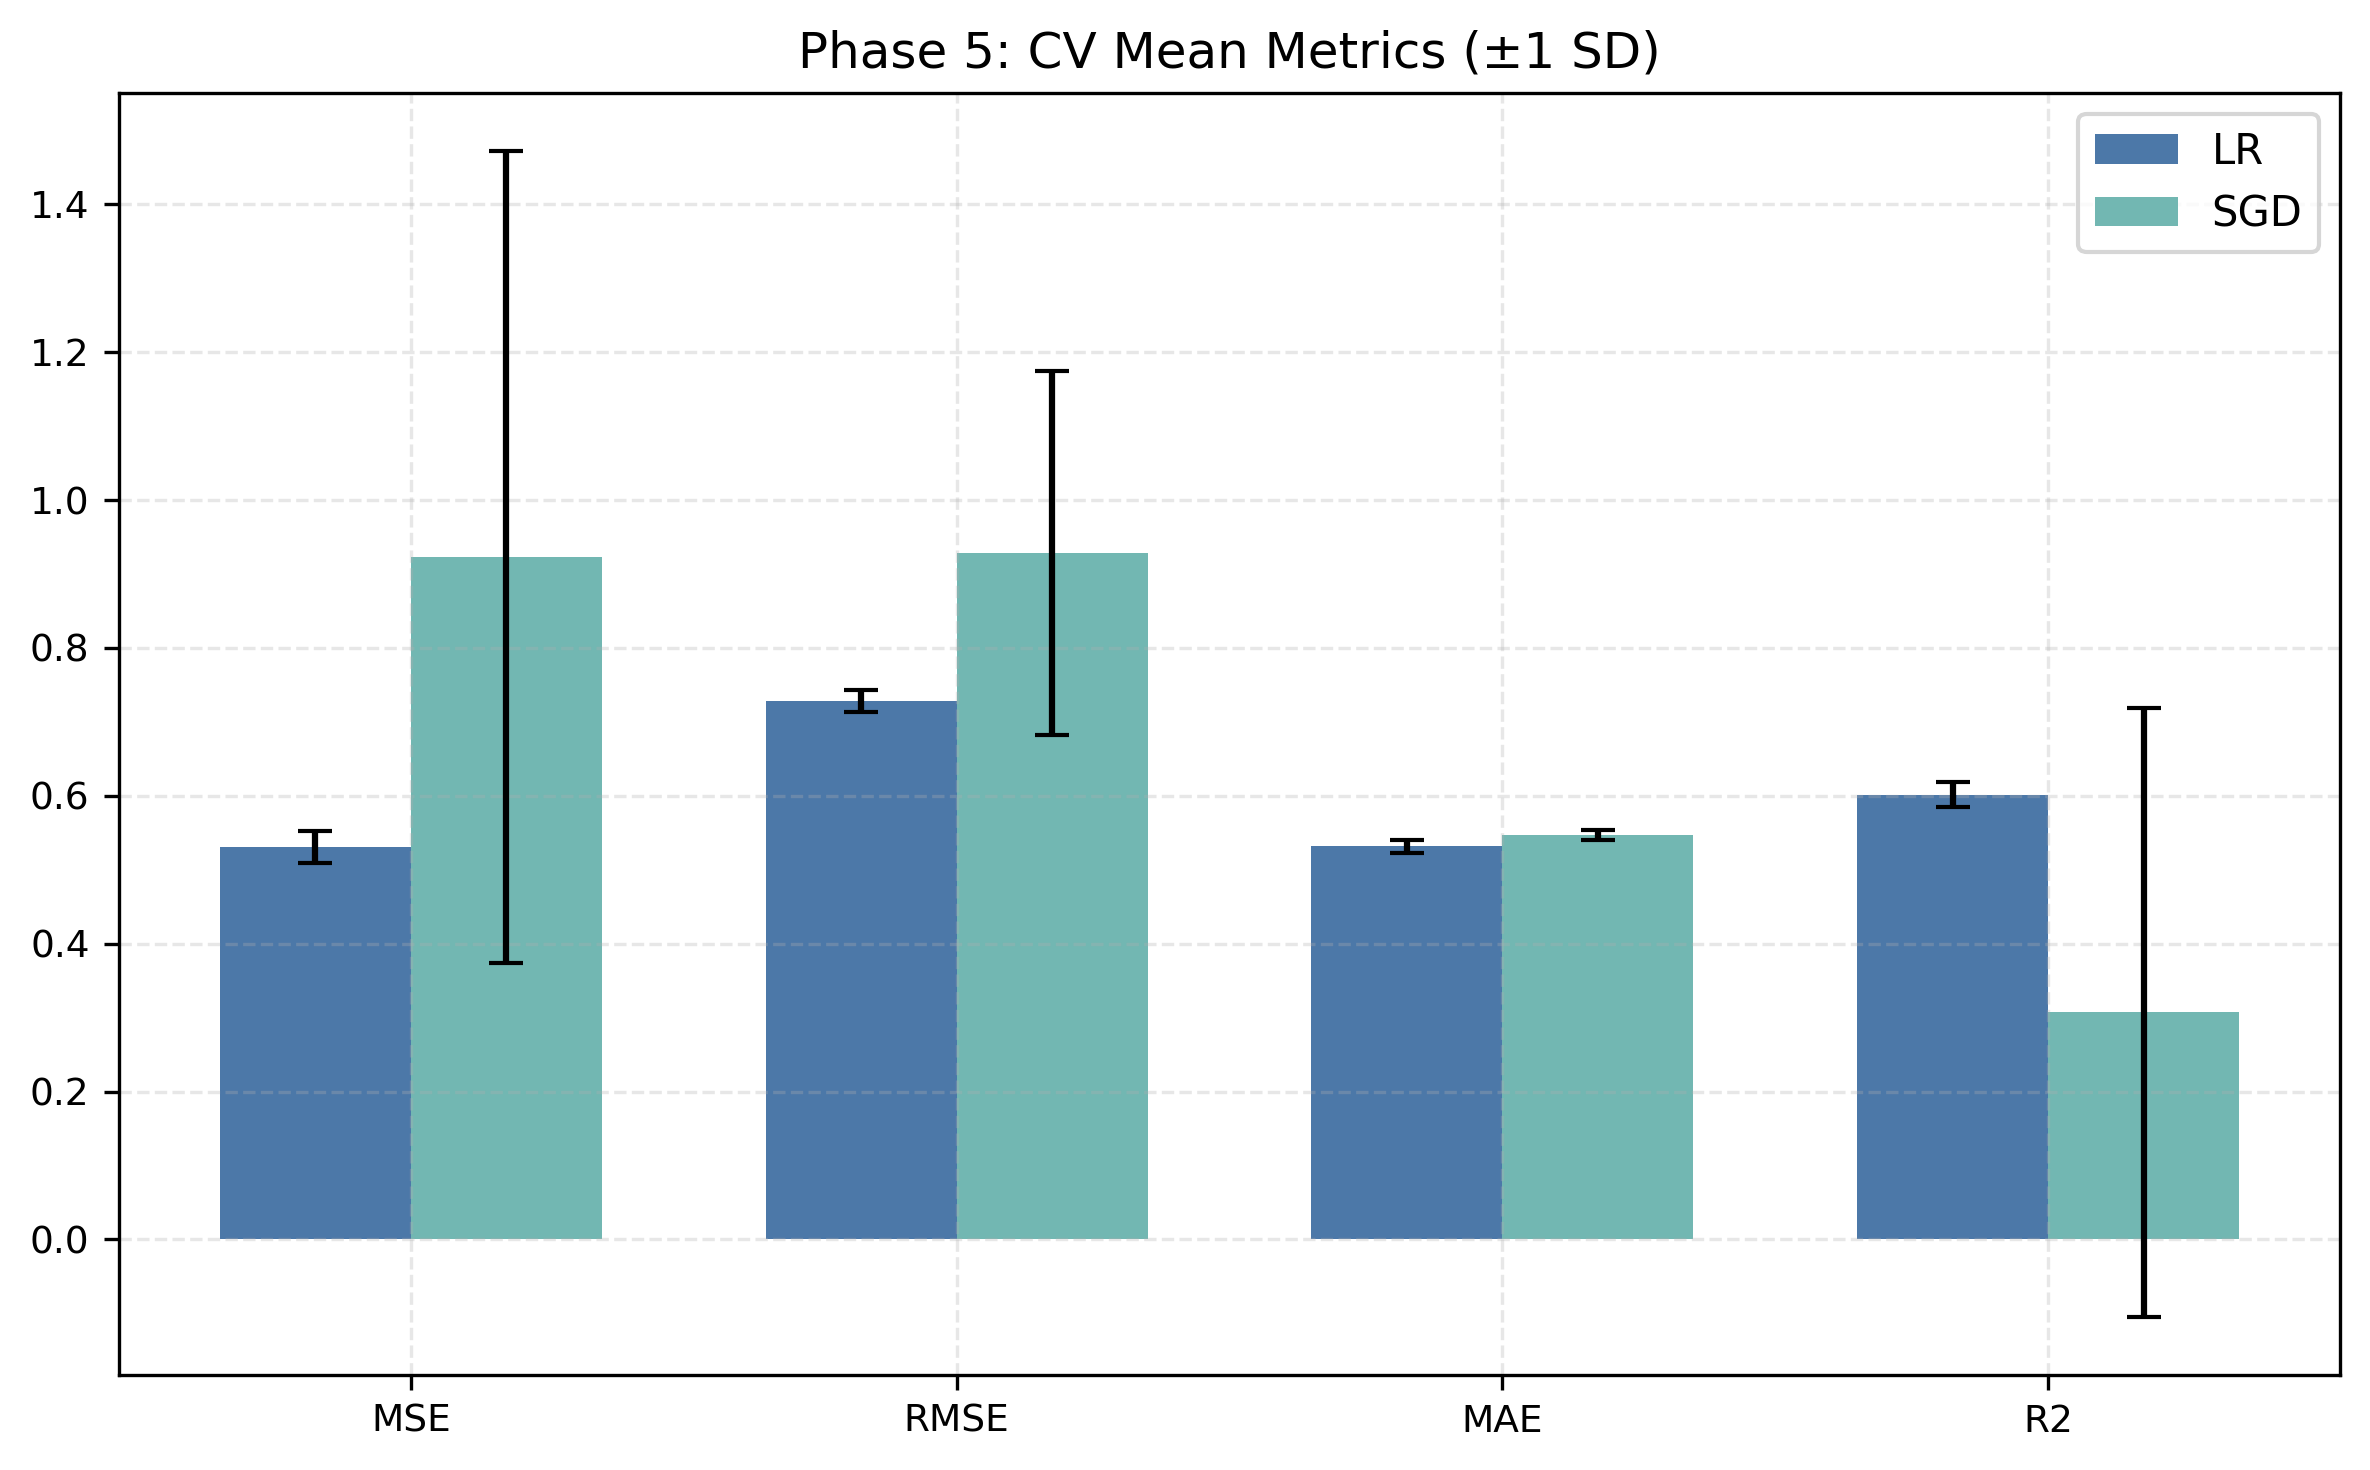
\includegraphics[width=0.95\linewidth]{data/Phase 5 CV Mean Metrics.png}
  \caption{Phase 5: CV mean metrics with error bars ($\pm$ 1 SD).}
  \label{fig:phase5-cv}
\end{figure}

\begin{table}[H]
  \centering
  \caption{Phase 5: 5-fold CV results (mean $\pm$ std).}
  \label{tab:phase5}
  \begin{tabular}{lcccc}
    \toprule
    Model & MSE & RMSE & MAE & $R^2$ \\
    \midrule
    LR  & $0.5306 \pm 0.0218$ & $0.7283 \pm 0.0149$ & $0.5317 \pm 0.0084$ & $0.6014 \pm 0.0170$ \\
    SGD & $0.9230 \pm 0.5489$ & $0.9285 \pm 0.2467$ & $0.5473 \pm 0.0069$ & $0.3070 \pm 0.4114$ \\
    \bottomrule
  \end{tabular}
\end{table}

\section{Results and Discussion}
Our experimental results demonstrate that LR and properly scaled SGD achieve comparable performance on the original feature set, with LR showing slightly better in-sample fit but similar generalization. Polynomial feature expansions substantially improve in-sample fit, particularly for LR (achieving $R^2 = 0.7287$ at degree 3), but introduce increased model complexity and potential overfitting risk. The modest train-test gaps for degree 1 models (7.3\% for LR, 4.2\% for SGD) contrast with the larger in-sample gains from higher-degree polynomials, suggesting that simpler models may be preferable for deployment.

Cross-validation results strongly favor LR for reliability, with tight variance across folds compared to SGD's high variability. Feature scaling proved essential for SGD convergence; without standardization, we consistently observed divergence and noisy training plateaus. The robust Huber loss and early stopping further stabilized SGD training. The strong positive correlation between \texttt{MedInc} and the target ($r = 0.6881$) explains why this single feature captures nearly half the variance, while the remaining features provide incremental improvements when combined.

\section{Conclusion}
We have demonstrated a complete NumPy-based pipeline for linear regression modeling on the California Housing dataset, systematically evaluating single-feature and multi-feature approaches through five experimental phases. Our results confirm that proper feature scaling and hyperparameter selection are critical for SGD performance, while polynomial expansions offer improved in-sample fit at the cost of increased variance and complexity. Cross-validation reveals that LR provides more stable and reliable predictions than SGD for this regression task. Future work should explore regularized models (Ridge, Lasso) to control overfitting in polynomial feature spaces, feature selection techniques to identify optimal subsets, and more sophisticated hyperparameter optimization for SGD under cross-validation.

\end{document}